\documentclass[tikz,border=10pt]{standalone}
% No extra TikZ libraries are needed for this figure.
\begin{document}
% Stroke width raised to 2pt per repair instruction
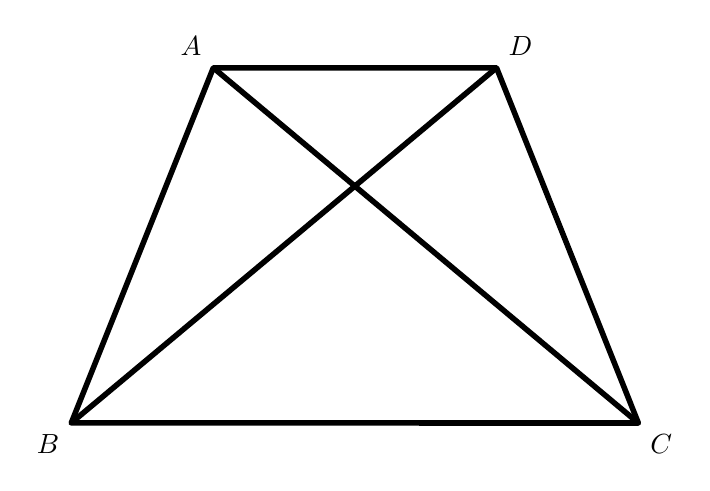
\begin{tikzpicture}[line join=round, line width=2pt]
  % Vertices, converted from pixels with s = 0.019093 and y flipped
  % (centre of ink bbox at px (259.5, 196))
  \coordinate (A) at (-1.6090004205273813,2.272198978814017);
  \coordinate (D) at (1.9880004205273816,2.2718010211859827);
  \coordinate (B) at (-3.412999789964224,-2.238101599944418);
  \coordinate (C) at (3.7889997899642243,-2.238898400055583);

  % Trapezoid sides: top AD, bottom BC, legs AB and DC
  \draw[solid, black] (A) -- (D) -- (C) -- (B) -- cycle;

  % Diagonals AC and BD (they cross inside the figure)
  \draw[solid, black] (A) -- (C);
  \draw[solid, black] (B) -- (D);

  % Vertex labels: \large, same placement as v1
  \node[above left]  at (A) {$\large A$};
  \node[above right] at (D) {$\large D$};
  \node[below left]  at (B) {$\large B$};
  \node[below right] at (C) {$\large C$};
\end{tikzpicture}
\end{document}